\chapter{Demo}\label{cap:demo}
Per illustrare il funzionamento dell'algoritmo, è stata realizzata una demo interattiva utilizzando la libreria Python \texttt{Gradio}. Gradio consente di avviare un web server locale con un'interfaccia grafica accessibile da browser, collegata direttamente a funzioni Python, permettendo di testare il modello in modo semplice.

Come mostrato in figura~\ref{fig:demo-general}, l'interfaccia guida l'utente attraverso le tre fasi principali:
\begin{enumerate}
    \item Caricamento dell'immagine.
    \item Pre-processing.
    \item Riconoscimento (OCR).
\end{enumerate}
\begin{figure}[H]
    \centering
    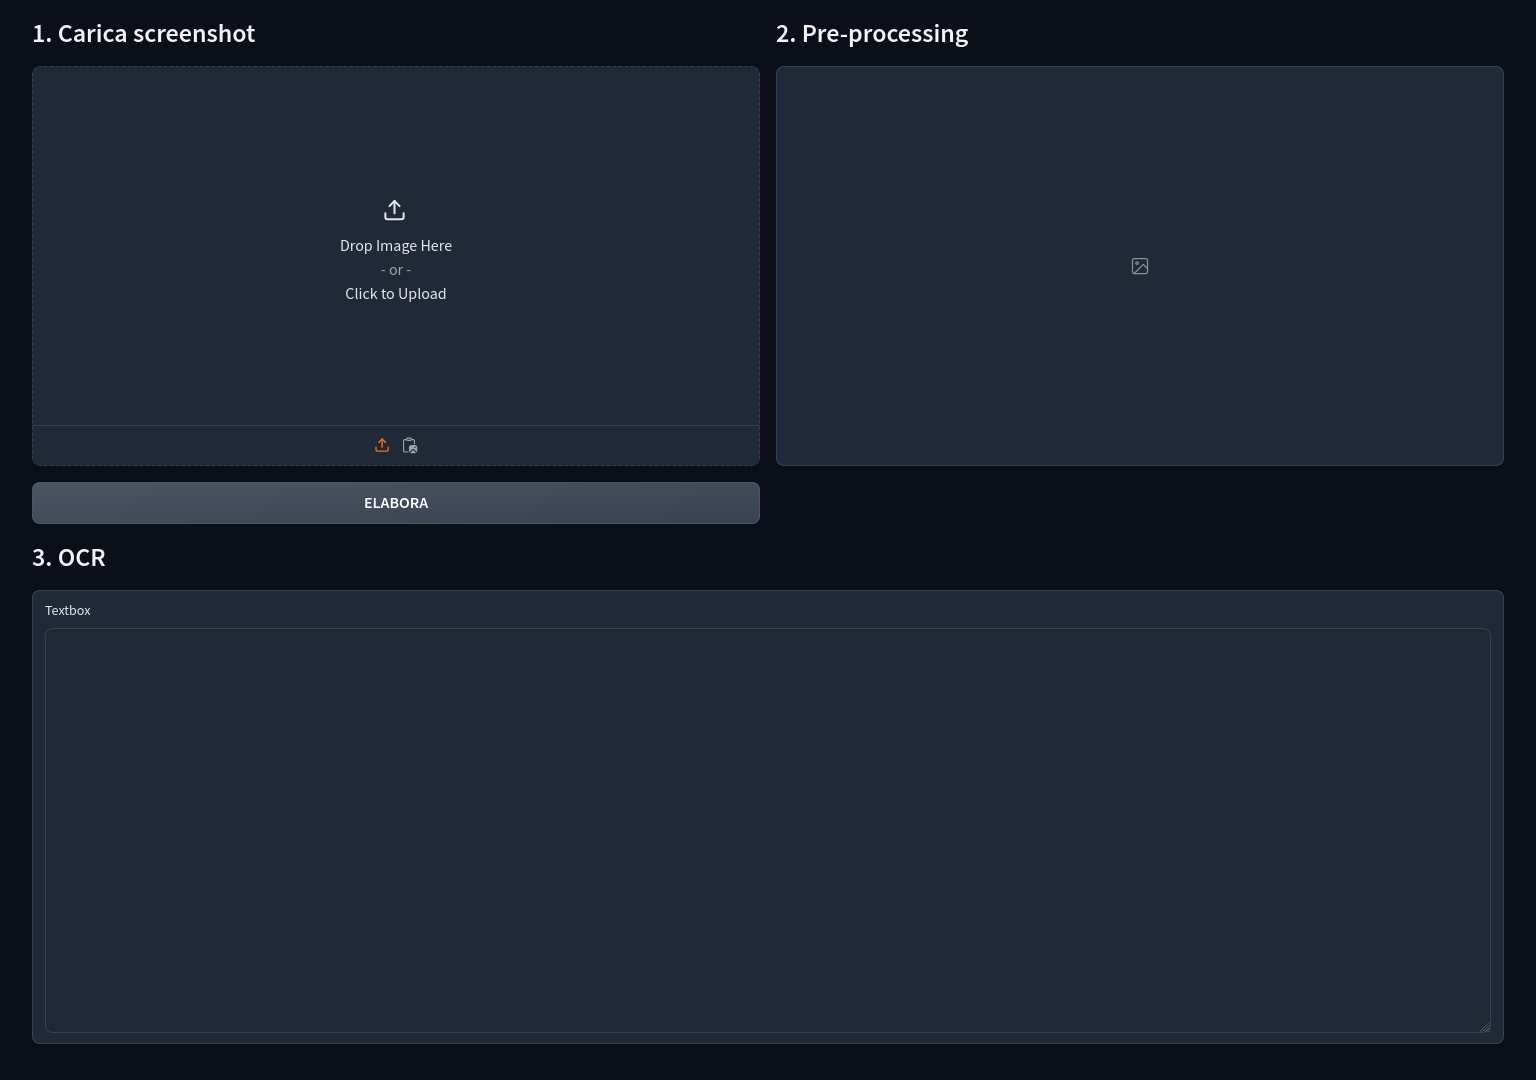
\includegraphics[width=0.7\textwidth]{images/demo_ui.png}
    \caption{Interfaccia della demo}
    \label{fig:demo-general}
\end{figure}

\subsection*{Caricamento dell'immagine}
In questa fase l'utente può caricare un'immagine da elaborare, selezionandola direttamente da una cartella oppure incollandola dalla clipboard.
\begin{figure}[H]
    \centering
    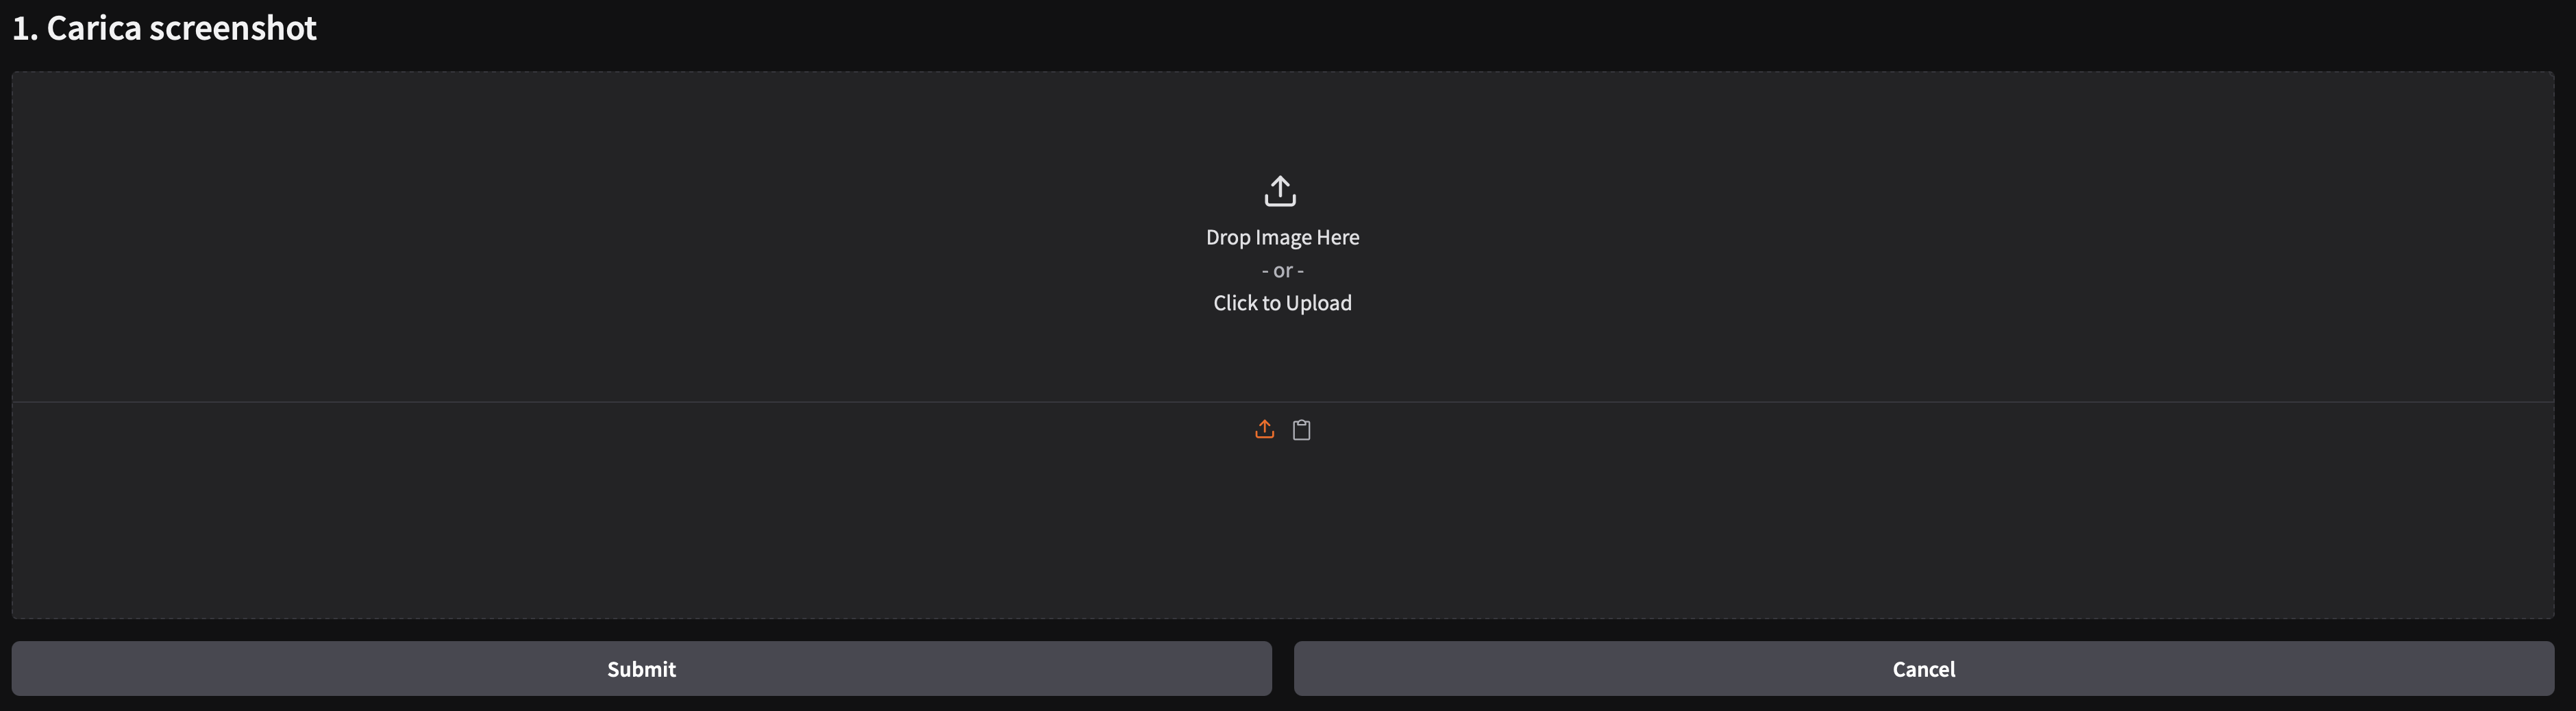
\includegraphics[width=0.7\textwidth]{images/demo-1fase.png}
    \caption{Interfaccia di caricamento dell'immagine}
    \label{fig:demo-1fase}
\end{figure}

\subsection*{Pre-processing}
Una volta cliccato il pulsante \texttt{ELABORA}, viene avviato il pre-processing dell'immagine. In output vengono mostrati due tipi di bounding box: uno \textbf{rosso} che delimita l'intera frase, e uno \textbf{verde} per ciascun carattere.

\begin{figure}[H]
    \centering
    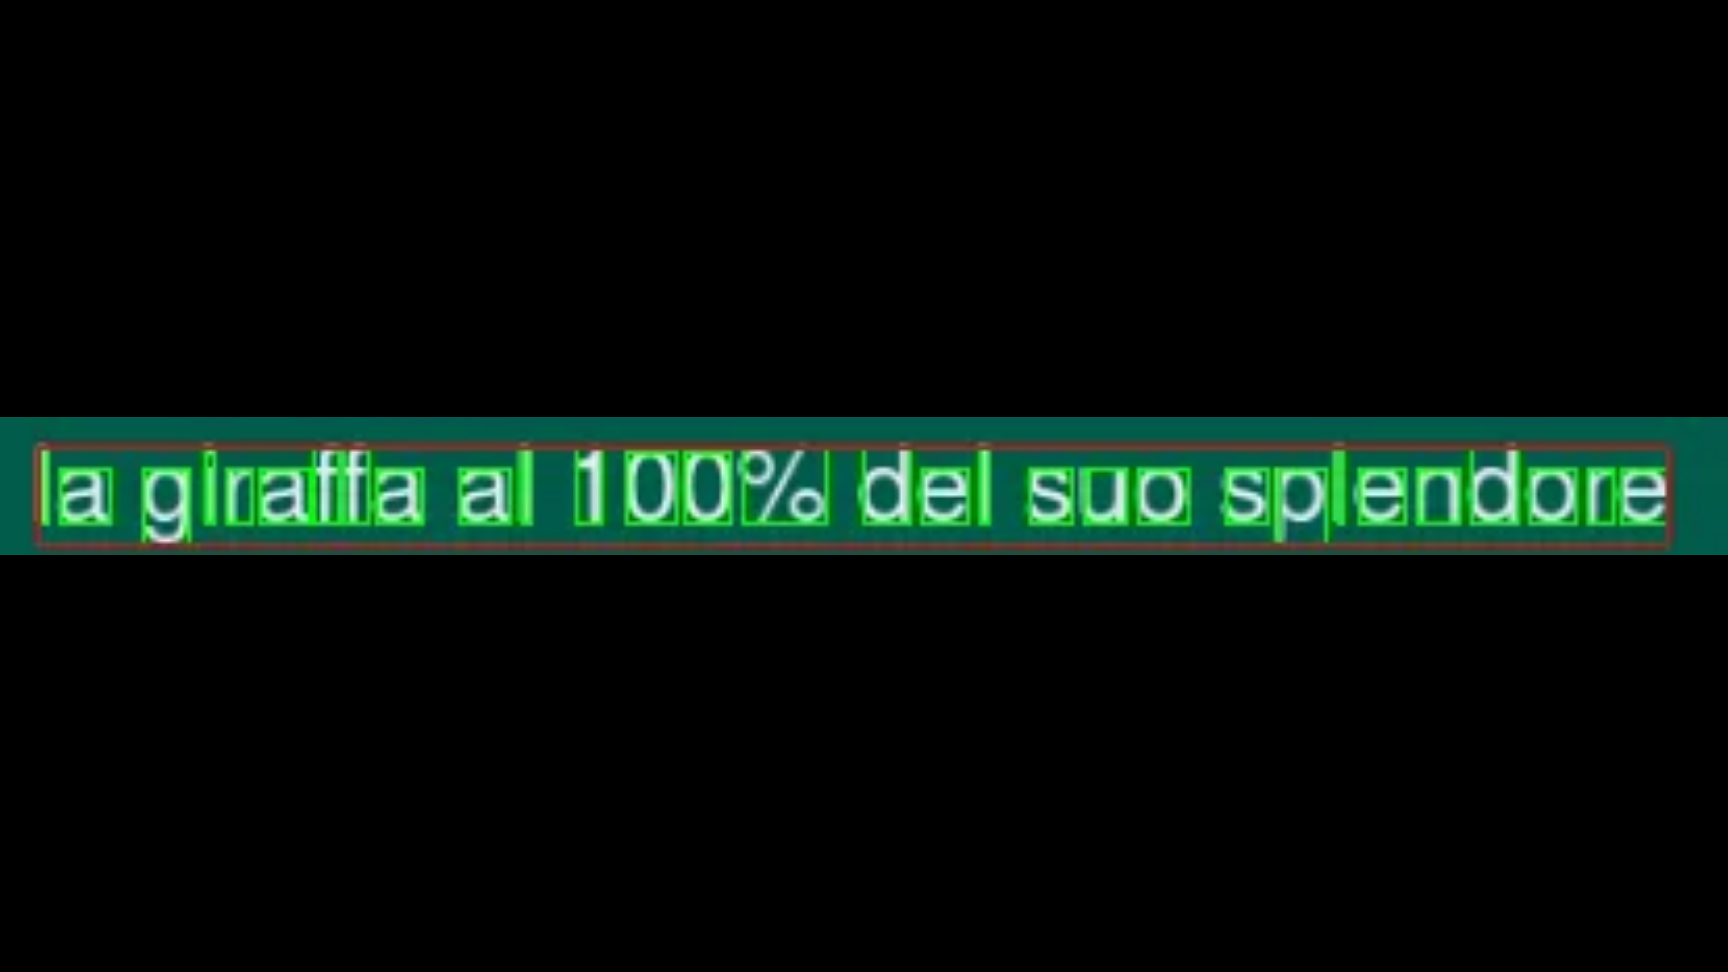
\includegraphics[width=0.7\textwidth]{images/demo-2fasedetail.png}
    \caption{Immagine pre-processata}
    \label{fig:demo-2fase}
\end{figure}

\subsection*{OCR}
Infine viene mostrato il testo riconosciuto dal modello
\begin{figure}[H]
    \centering
    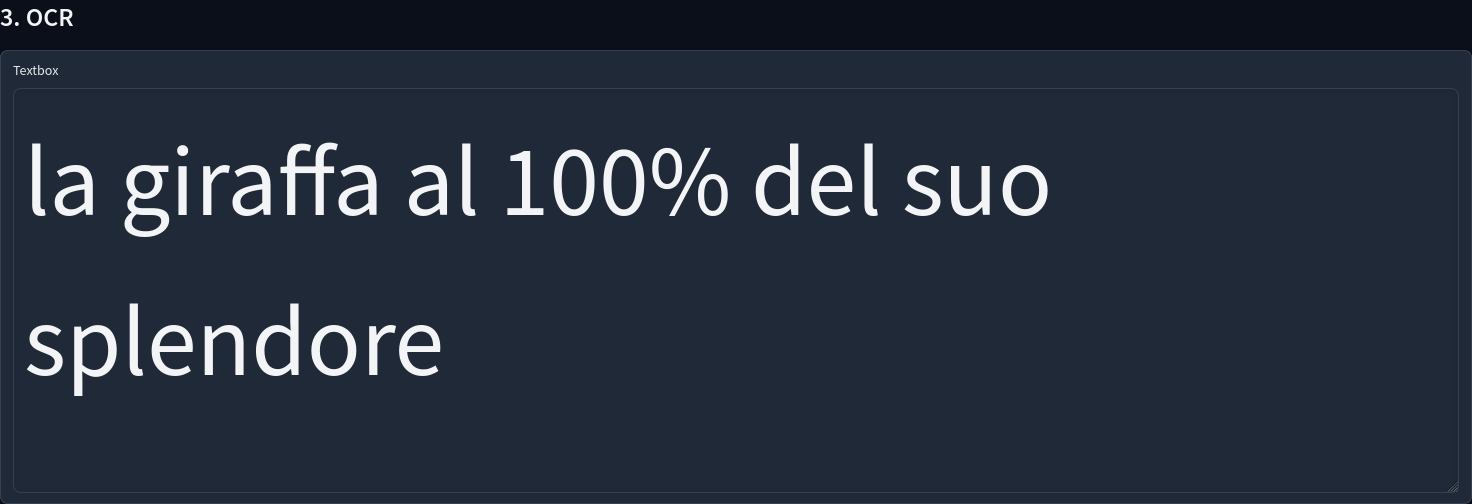
\includegraphics[width=0.7\textwidth]{images/demo-3fase.png}
    \caption{Output modello}
    \label{fig:demo-3fase}
\end{figure}

Per una dimostrazione completa del funzionamento della demo, è disponibile un video al \href{https://github.com/user-attachments/assets/c438a7b3-e5fd-433e-a72f-7376223e9067}{seguente link}.